% For printing in a4
%\documentclass[a4,10pt,twoside,openright,italian,english]{book}% twoside!

% For printing with the A5 format
\documentclass[11pt,twoside,openright,english,italian]{book}% twoside!

% Set paper size
\usepackage[twoside=true]{geometry}

\geometry{a4paper,
  top=33mm,
  bottom=34mm,
  inner=38mm,
  outer=32mm,
  bindingoffset=5mm
}

%\usepackage[cam,center,a4,pdflatex,axes]{crop}

\usepackage{phdthesis}
\usepackage{phdtitle}



\usepackage{listings}
\usepackage{subfig}
\usepackage{graphicx}
\usepackage{xcolor}
\usepackage{bibentry}
\usepackage{setspace}
\usepackage[english,italian]{babel}
\usepackage[toc]{appendix}
\usepackage[bookmarks=true,pdftex=false,bookmarksopen=true,pdfborder={0,0,0},hidelinks]{hyperref}
%\usepackage{array}
%\usepackage{epstopdf}
%\usepackage{color}
%\usepackage{mdwmath}
%\usepackage{mdwtab}
%\usepackage{amsmath,amssymb}
%\usepackage{cite}
%\usepackage{glossaries}
%\usepackage{booktabs}
%\usepackage{latexsym}
%\usepackage{url}
%\usepackage{bnf}
%\usepackage{rotating}
%\usepackage{multirow}
%\usepackage{paralist}
%\usepackage[algochapter]{algorithm2e}
%\usepackage{lscape}
%\usepackage{algorithmic}
%\usepackage{algorithm}
%\usepackage{longtable}
%\usepackage[T1]{fontenc} 
%\usepackage[utf8]{inputenc}

\hyphenation{}

\onehalfspacing

\lstset{tabsize=2,basicstyle=\footnotesize,breaklines=true}

\hypersetup{pdftitle={Title}, pdfauthor={Paolo Paterna}}

\nobibliography*

\department {Scuola di Ingegneria Industriale e dell'Informazione}
\phdprogram{Tesi di Laurea Magistrale in\\Computer Science and Engineering}

\author{Paolo Paterna}
\authorid{852548}

\title{Title}
\supervisor{Raffaela Mirandola}
\tutor{Diego Perez-Palacin}
\titleimage{img/logo_poli.eps}
\phdcycle{A.Y. 2017/2018}

%%%%%%%%%%%%%%%%%%%%%%%%%%%%%%%%%%%%%%
% Let's Start The Real Document
%%%%%%%%%%%%%%%%%%%%%%%%%%%%%%%%%%%%%%
\begin{document}
\selectlanguage{english}

\maketitle

\cleardoublepage

% change numbering into Roman numbers for the introductory part
\setcounter{page}{1}
\pagenumbering{Roman}

%%%%%%%%%%%%%%%%%%%%%%%%%%%%%%%%%%%%%%
% TOC
%%%%%%%%%%%%%%%%%%%%%%%%%%%%%%%%%%%%%%
\setcounter{tocdepth}{1}
\tableofcontents
\cleardoublepage


%
% LIST OF 
%
\addcontentsline{toc}{chapter}{List of Figures}
\listoffigures
\addcontentsline{toc}{chapter}{List of Tables}
\listoftables


%%%%%%%%%%%%%%%%%%%%%%%%%%%%%%%%%%%%%%
% Acknowledgement
%%%%%%%%%%%%%%%%%%%%%%%%%%%%%%%%%%%%%%
\addcontentsline{toc}{chapter}{Acknowledgment}
\chapter*{Acknowledgments}
\iffalse
I would like to thank my thesis supervisor \emph{prof. William Fornaciari} and
my thesis co-supervisor \emph{Giuseppe Massari} for the time dedicated to
guide me on the process of researching and writing this thesis. I would also
like to thank \emph{Simone Libutti} and \emph{Gianmario Pozzi} for the help in
the development of work proposed in this thesis.

\vspace{0.5cm}

I would like to acknowledge the invaluable support provided by the \emph{CRIU}
and \emph{Open MPI} developers for the provided advices on the code
integration proposed in this work. I would also to thank the IT4Innovations
(IT4I) supercomputing center\footnote{https://www.it4i.cz/} and its experts for
providing us the systems for performing the experimental evaluations.

\vspace{0.5cm}

Finally, I would like to express my deep gratitude to my parents \emph{Manuela}
and \emph{Mauro} and my girlfriend \emph{Lara} for providing me unfailing
encouragement during these years of study and thesis writing.

\vspace{0.5cm}

This accomplishment would not have been possible without the support of the
previously mentioned people. Thank you.
\fi
\cleardoublepage

%%%%%%%%%%%%%%%%%%%%%%%%%%%%%%%%%%%%%%
% Abstract
%%%%%%%%%%%%%%%%%%%%%%%%%%%%%%%%%%%%%%
% MAX 2200 CARATTERI!
\addcontentsline{toc}{chapter}{Abstract (Italian version)}
\chapter*{Abstract (Italian version)}
\markboth{Abstract (Italian version)}{}

\begin{otherlanguage}{italian}

\lettrine{I}{} sistemi High Performance Computing (HPC) sono tipicamente
caratterizzati da
un gran numero di risorse - CPU, GPU, ecc - implicando, di conseguenza, la necessità di
affrontare il problema di una loro efficace utilizzazione. In aggiunta a ciò, non
è possibile ignorare le strategie di risparmio energetico e dissipazione del calore essenziali in ambiente HPC.
Questo quadro è reso ancora più complesso dal fatto che i moderni
sistemi sono caratterizzati da un livello decrescente di affidabilità.
Per tutte queste ragioni, meccanismi e politiche poco invasive
di gestione delle risorse diventano essenziali al fine di risolvere i problemi presentati.

Proprio a causa della loro natura distribuita, i sistemi HPC utilizzano
paradigmi di programmazione
parallela, tra i quali annoveriamo uno dei più utilizzati: Message Passing
Interface (MPI). Questa tesi presenta un'estensione dell'implementazione
Open MPI, chiamata \texttt{mig}, al fine di supportare in modo trasparente
la migrazione di processi di un'applicazione.

Questo meccanismo è integrabile con un gestore delle risorse
e in questo lavoro ne viene proposto uno basato su Barbeque
Run-Time Resource Manager. Questo approccio ci consente di superare la
limitazione di MPI che impedisce la ridefinizione dell'assegnamento delle risorse computazionali a runtime una volta che l'applicazione è stata lanciata. Ciò
rappresenta anche una limitazione sia per quanto concerne l'implementazione di strategie di resilienza ai guasti, sia nei riguardi dell'uso efficace delle risorse. 

L'estensione \texttt{mig} aumenta la flessibilità introducendo una granularità
più fine di allocazione del carico di lavoro, attraverso la possibilità di
eseguire la \emph{migrazione dei processi}. A tal proposito, in letteratura esistono già molte tecniche di migrazione, ma mancano principalmente
di trasparenza
rispetto all'applicazione. In passato in Open MPI esisteva un supporto per la
tolleranza ai guasti basato su tecniche di Checkpoint/Restart, ma fu
successivamente rimosso a causa della difficile manutenibilità.

In questa tesi proponiamo il framework \texttt{mig} come un'estensione di
Open MPI per risolvere i problemi precedentemente descritti, in particolare
in termini di
trasparenza e manutenibilità. L'implementazione di una politica di allocazione
delle risorse per BarbequeRTRM è proposta come un possibile caso d'uso del framework.


\end{otherlanguage}

\addcontentsline{toc}{chapter}{Abstract}
\chapter*{Abstract}
\markboth{Abstract}{}

\lettrine{T}{he} High Performance Computing (HPC) systems typically include
a large number of computing resources - CPUs, GPUs, etc. As a consequence,
we must face with the problem of an effective utilization of them. In addition,
we cannot avoid from taking into account power saving and thermal management
strategies. The overall picture is made more complex by the fact that modern
systems are affected by decreasing level of reliability. For all these reasons,
we need effective and poorly invasive resource management mechanisms and
policies to address these issues.

Moreover, HPC systems need specific parallel programming paradigms, among these one of
the most widespread is Message Passing Interface (MPI). This thesis presents
an extension of the Open MPI implementation, called \texttt{mig} to
transparently support
the migration of application processes. This mechanism may be driven by a
resource manager and in this work an example of exploitation based on the
Barbeque Run-Time Resource Manager is proposed. This approach allows us also
to overcome a limitation of the MPI paradigm. In fact, once the application is
launched it is no more possible to redefine the assignment of computing
resource at run-time. This represents also limitation from the point of view of
effective usage of the resources and implementation of fault-tolerance
strategies.

The \texttt{mig} extension introduces more flexibility by enabling a more fine grained workload allocation, through the possibility of performing
\emph{process migration}. In this regard, a lot of  migration techniques are already available
in  literature, but they suffer from the lack of
transparency with respect to the application. In the past, Open MPI had
fault-tolerance support based on Checkpoint/Restart techniques, but they were subsequently removed due to hard maintainability requirements.

In this thesis we propose the \texttt{mig} framework as an Open MPI extension
that overcomes the aforementioned issues in terms of transparency and poor
maintainability. The implementation of a resource allocation policy for the
BarbequeRTRM is also proposed as an example of exploitation of the framework.

\cleardoublepage

% Now lets go back to normal numbering
\setcounter{page}{1}
\pagenumbering{arabic}

\chapter{Introduction}
\label{cap:introduction}

\section{The evolution of HPC systems}
\textbf{High Performance Computing (HPC)} term refers to computer technologies
used in advanced software applications requiring large computing power. The
applications are usually parallel in order to run on large clusters of
machines, called \textbf{supercomputers}.

HPC systems are currently considered one
of the most important resources both in research and in industry; the raising
of performance-hungry scientific applications lead European Union and other
subjects to allocate huge amount of funds to HPC development. HPC is 
considered strategic
for Europe's future and essential for industry to innovate in products and
services \cite{EUstrategy}. However, the research is called to solve several
technological limits to the performance scaling, along with addressing
the problem of providing guarantees in terms system reliability too, as
described in the subsequent paragraphs.

The increasing number of computing nodes, thus CPU cores, the end of
Dennard's scaling \cite{esmaeilzadeh2011dark} and the moving towards Exascale
computing\footnote{see next section for the Exascale definition.} indeed
introduce numerous challenges, in particular regarding thermal and energy
optimizations, dependability and resilience concerns, resource allocation
scheduling, and parallel programming models \cite{shalf2010exascale}.

Currently, the main component of HPC infrastructure variable costs is related
to thermal and energy considerations. More power consumption means more
electricity costs and heat dissipation, more heat dissipation means higher
cooling needs and consequently again more electricity costs. Considering the
large numbers of servers in HPC clusters, introducing an optimization in a
small part of the system may lead to not negligible economical
and environmental advantages. In fact, Exascale requires strong efforts in all
related fields, from the infrastructure to the software in the direction of
increasing power efficiency and programmability.

\begin{figure}[t]
		\centerline 
{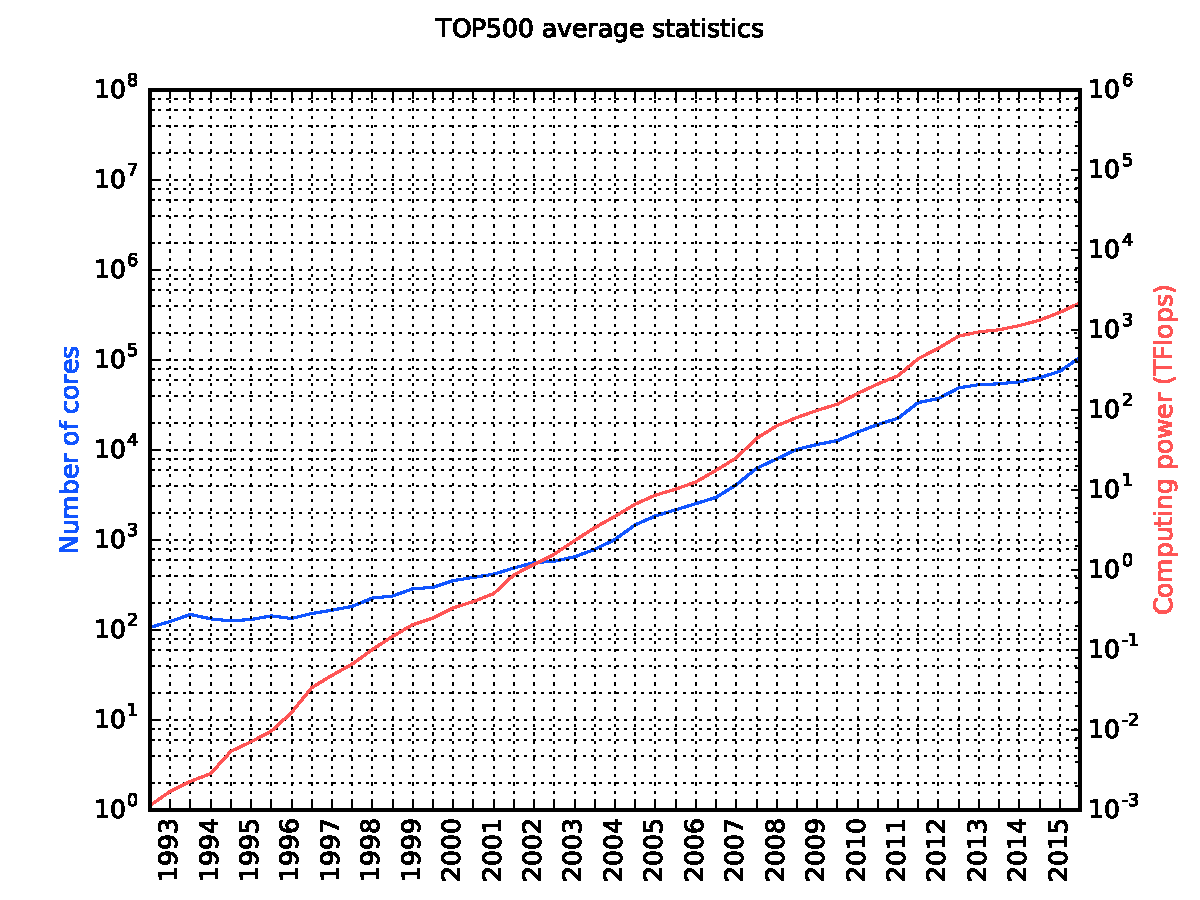
\includegraphics[scale=0.7]{img/cap1-top500-avg-comp}}
		\caption[TOP-500 supercomputers average performance]{Average number of cores and computing power of TOP-500
		supercomputers (TOP500.org data, retrieved 5 August 2016)}
		\label{fig:corestrend}
\end{figure}

\begin{figure}[t]
		\centerline 
{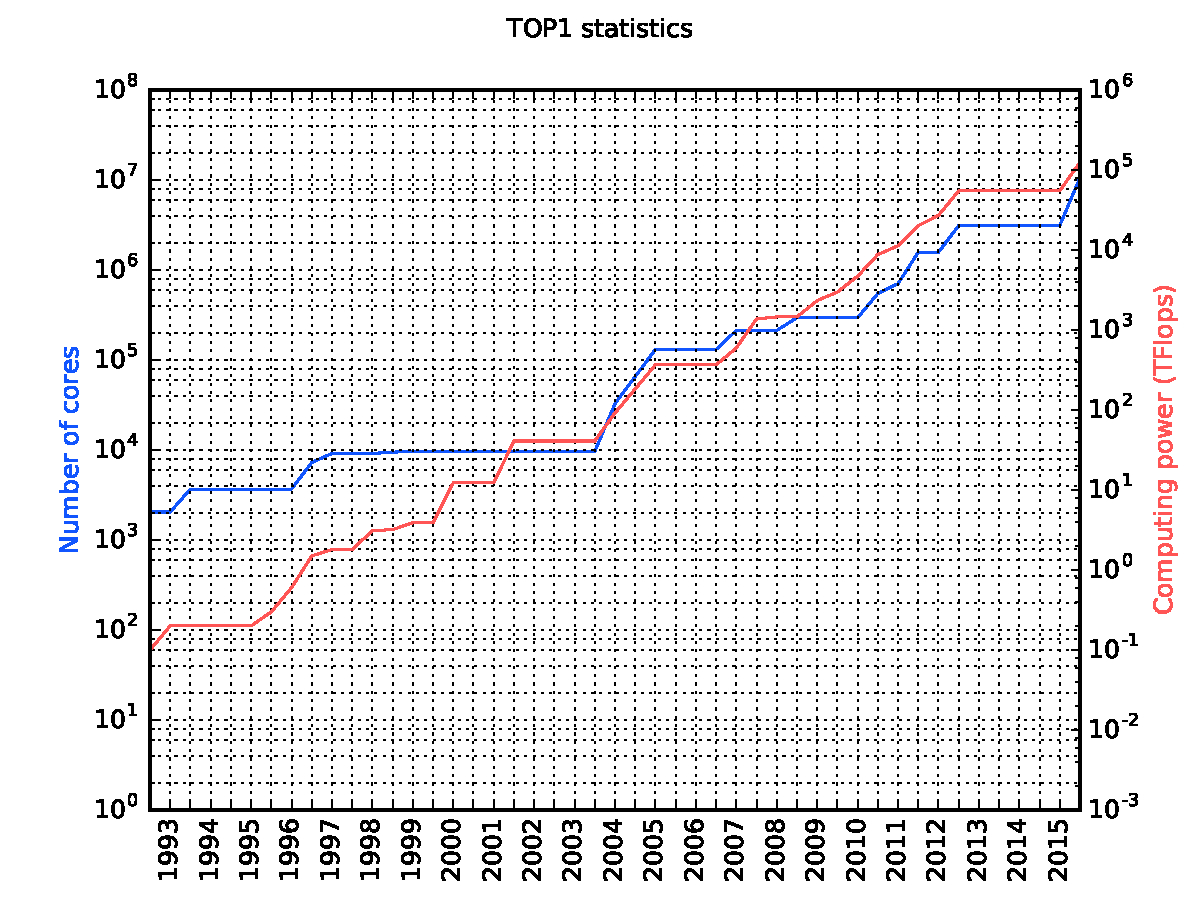
\includegraphics[scale=0.7]{img/cap1-top500-max-comp}}
		\caption[TOP-1 supercomputers performance]{Number of cores and computing power of the TOP-1
		supercomputer (TOP500.org data, retrieved 5 August 2016)}
		\label{fig:corestrend2}
\end{figure}


In last decades the rapid development of processing units maintained
acceptable levels of power consumption while increasing the performance
delivered. The computational units and computational power trends over
past two decades is shown in Figure \ref{fig:corestrend} and Figure
\ref{fig:corestrend2}.

Unfortunately, the miniaturization of semiconductors cannot go on forever,
thus the End of the \emph{Moore's Law} is one of the big concern. In fact,
the plateauing of voltage levels and the increasing of leaking current is
leading to a power wall \cite{Villa2014}.
The reduction of the performance increasing
trend, or even the reaching of a performance plateau, would significantly slow
down the scientific research \cite{snir2011exascale}. In 2014, the Department
of Energy of United States planned to achieve the too ambitious goal of
Exascale with 20 MW of power in 2018 \cite{USExascale}, but later the deadline
was extended.

\subsection{Exascale as a key goal to reach}
\textbf{Exascale computing} refers to systems having a minimum computing power
of more than 1 exaFLOPS, i.e. \( 10^{18} \) FLOPS.

Research towards Exascale is not limited to the computer science domain, but it
strongly affects all the areas of science and engineering. The increasing
complexity of mathematical models and the growing size of Big Data requires
a growing amount of computing resources.

The Exascale goal is in fact of great interest for a wide range of
applications. We can mention several examples, like the study of astrophysical phenomena, weather forecasting, product market simulations, the development of
new drugs, the analysis of health risks, etc.
\cite{Reed:2015:ECB:2797100.2699414}. For all these applications, Exascale
would enable the possibility of deploying more complex mathematical models,
capable of providing much more accurate and reliable results.


%%%%%%%%%%%%%%%%%%%%%%%%%%%%%%%%%%%%%%%%%%%%%%%%%%%%%%%%%%%%%%%%%%%%%%%%%%%%%%%
Vice versa, other non-computer scientists
are studying to find alternative technologies to the current one, in order to
mitigate the today issues. Several physicist are studying new types of
semiconductors, for instance the very promising research on silicon photonics
\cite{6476868}.

From the previous considerations we can state that HPC is still a very hot
topic of research and solving the related problematics is not just a matter
of computer science, but it will influence and it will be influenced by
the research activities in almost all fields.

%%%%%%%%%%%%%%%%%%%%%%%%%%%%%%%%%%%%%%%%%%%%%%%%%%%%%%%%%%%%%%%%%%%%%%%%%%%%%%%


\subsection{HPC systems architecture}
Since HPC systems require by definition high computational capabilities, the
computational resources are typically distributed across different high-end
machines (nodes). They are connected via a high speed networks, typically
10Gigabit Fiber Optics Ethernet or InfiniBand.

The storage is also provided through distribution solutions like
Storage Area Network (SAN) or Network Attached Storage (NAS).
Both solutions have to be designed for
HPC environment. In particular, the storage performance and capacity
should possibly scale linearly with the numbers of nodes and disks.

\begin{figure}[t]
		\centerline 
{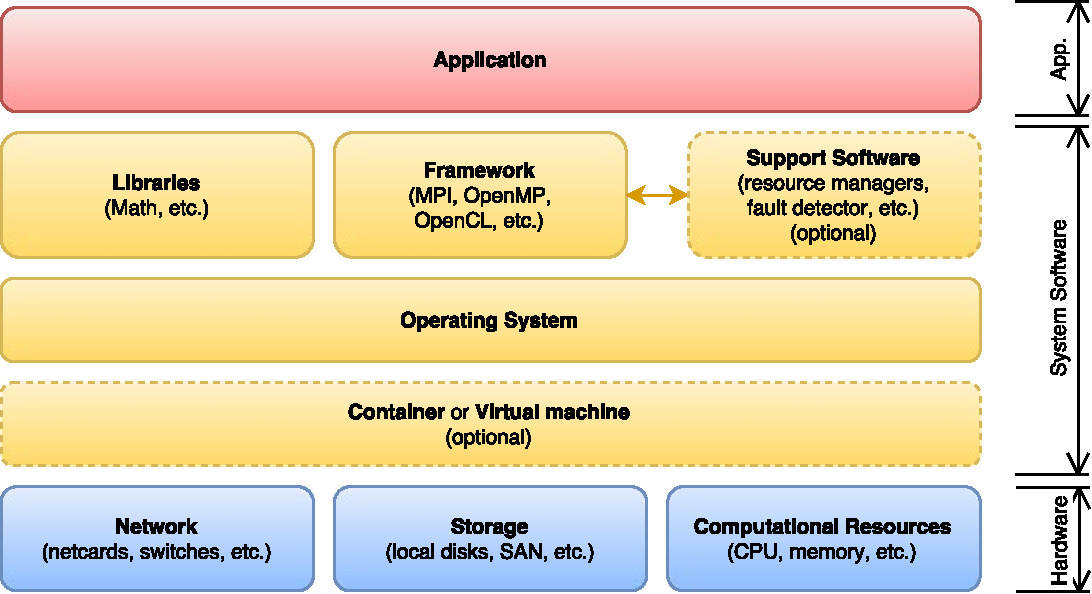
\includegraphics[scale=0.7]{img/cap1-generalarchitecture.pdf}}
		\caption[General architecture of a HPC node]{The general architecture of one node in a HPC system.}
		\label{fig:generalarchitecture}
\end{figure}

The general architecture of a single node in a HPC cluster is shown in
Figure \ref{fig:generalarchitecture}. End-user applications run over
a stack of software and, in particular, exploit the API provided
by a specific parallel programming framework like MPI or OpenMP. Since the
application computational requirements are far behind the performance
capabilities provided by a single CPU, the application must be designed in
order to run multiple threads or processes. Parallel frameworks
simplify the development of the applications, providing suitable API to
manage the execution of multiple tasks, the communication and the
synchronization among them.

Furthermore, the application may use other library providing specific
functionalities (e.g. math functions) or interact with
other software frameworks, like resource managers. The operating system as
usual provides to all of software the abstraction of the hardware (virtualized
or not).


\section{Dependability issues in HPC}
In HPC, dependability - a broad term including reliability, resilience,
fault tolerance, etc. - is another possible future wall in reaching
Exascale computing \cite{5871590}. To highlight the
size of the problem is sufficient to say that the Mean Time To Failure (MTTF)
for current HPC systems is way below 100 hours \cite{egwutuoha2013survey}.

The research community is therefore focusing its effort towards five key
directions \cite{cappello2014toward}:
\begin{enumerate}
\item statistical and technical characterization of hardware faults;
\item development of a standard fault interface from hardware to software;
\item improving fault prediction, containment, detection, notification and recovery;
\item the development of programming abstractions for resilience, especially fault-tolerant algorithms;
\item proposing fault-tolerant approaches both in hardware and software design.
\end{enumerate}

In this work, we focus on the item 4 proposing a tool that can be used
in HPC parallel applications in conjunction with a fault-detection mechanism to
support fault-tolerant executions on distributed systems.


\subsection{Fault-Tolerance requirements and techniques}
As already presented, one of the most important discussed theme in HPC is the
dependability concern. In particular, since the MTBF is very low compared
to the applications timespan, it is required fault-tolerance techniques
able to guarantee the termination of the application even if one or more faults
occur. In fact, some HPC applications take days or weeks to terminate and
after a fault a restart from the beginning is not acceptable. Therefore,
fault-tolerance is no longer a \emph{nice-to-have} feature, but it became a
\emph{mandatory} one in HPC systems.

To highlight the previous considerations, a simplification of
the Mean Time To Failure (MTTF) and Mean Time Between Failure calculus (MTBF)
is proposed, with the objective to provide a trivial qualitative analysis.
Assuming the system non repairable, thus \( \text{MTTF}=\text{MTBF} \),
let's consider a cluster of 1.000 CPUs Intel Xeon processor of E7 Family that has \(\text{MTTF}=100.000h\) (\textasciitilde 11y) \cite{E7Reliability}. The overall MTTF can be calculated as:

	\begin{equation}\label{eq:mttf1}
		\lambda_i = \frac{1}{\text{MTTF}_i}
	\end{equation}
	\begin{equation}\label{eq:mttf2}
		\lambda_{\text{overall}} = \sum{\lambda_i}^n
	\end{equation}
	\begin{equation}\label{eq:mttf3}
		\text{MTTF}_{\text{overall}} = \frac{1}{\lambda_{\text{overall}}}
	\end{equation}

Applying (\ref{eq:mttf1}), (\ref{eq:mttf2}), (\ref{eq:mttf3}) to our scenario:
\[  \text{MTTF}_{\text{overall}} = \frac{1}{ 1.000 \cdot \frac{1}{100.000} }
 = 100h \]

The overall MTTF was drastically reduced from 11 years to just few days.
Please also note that modern supercomputers have more than 30.000 physical
CPUs, leading to MTTF to be less than 4 hours. It is clear that most of the
HPC applications, that requires more than few hours to conclude, need a
sort of abstract of a fault-free system, in order to execute ideally without
being affected by hardware faults. Several approaches have been proposed in
literature and industry. The state of the art of this techniques will be
discussed in the next chapter.

\subsection{Failures taxonomy and sources}
Following the classification provided by \emph{Snir et al.}
\cite{snir2014addressing}, the HPC failures may be grouped in three
categories: \emph{detected and corrected by the hardware} (DCE), \emph{detected
but not corrected by the hardware} (DUE) and \emph{non-detected silent errors}
(SE).
We do not consider DCE, since they are transparent to the software; for
instance, the ECC memory correction is an example of DCE and it is usually
performed transparently to the software. We neither deal with SE: the
correctness of the result has to be checked by the application since the
framework has no tool to infer it.

In the example about the calculation of MTTF, the CPU fault rate was
considered. However, other components like memory may be the source of
the failure, further deteriorating the reliability. Regarding \textbf{hardware faults}, they can be divided -
following the \emph{Snir et al.} classification - in \emph{compute soft},
\emph{compute hard}, \emph{network}, and \emph{I/O} errors. Vice versa,
\textbf{software faults} can be classified in: \emph{pure software}, 
\emph{hardware propagating up}, and \emph{software propagating down} errors. 
This taxonomy is better presented in the subsequent 
Table \ref{tab:faulttaxonomy}.


\begin{table}[ht!b]
\centering
\begin{tabular}{ c|c|c}

\multirow{4}{*}{\parbox{2.5cm}{\vspace{2cm}Hardware faults}} 
 & \centering Compute soft errors & \parbox{6cm}{\vspace{.5\baselineskip}
 Errors caused by transient
 faults in electronics,  e.g. memory corruptions caused by an electromagnetic
 interference
 \vspace{.5\baselineskip}}
 \\ \cline{2-3}
 & \centering Compute hard errors & \parbox{6cm}{\vspace{.5\baselineskip}
 Permanent fault of a
 computational component (CPU, RAM, etc.) due to a physical problem, e.g.
 electromigration.
 \vspace{.5\baselineskip}}
 \\ \cline{2-3}
 & \centering Network errors & \parbox{6cm}{\vspace{.5\baselineskip}
 Total or partial loss of network
 connectivity, often caused by external component w.r.t. machine, e.g.
 network apparatus failures.
 \vspace{.5\baselineskip}}
 \\ \cline{2-3}
 & \centering I/O errors & \parbox{6cm}{\vspace{.5\baselineskip} Transient or
 systematic errors during
 the reading or writing to disks or other storage
 \vspace{.5\baselineskip}} \\ \hline
\multirow{3}{*}{\parbox{2.5cm}{\vspace{1.3cm}Software faults}} 
 & \centering Pure software errors & \parbox{6cm}{\vspace{.5\baselineskip}
 The category containing the
 classical programming issues: correctness errors, concurrency errors, etc.
 \vspace{.5\baselineskip}}
 \\ \cline{2-3}
 & \centering HW propagating to SW & \parbox{6cm}{\vspace{.5\baselineskip}
 A bug in the hardware that
 propagates up to the software, typical an unmanaged DUE.
 \vspace{.5\baselineskip}}\\ \cline{2-3}
 & \centering SW propagating to HW & \parbox{6cm}{\vspace{.5\baselineskip}
 A bug in the software that
 damages the hardware; it is typical of firmware in embedded appliances.
 \vspace{.5\baselineskip}}\\ 

\end{tabular}

\caption[The fault taxonomy in a HPC environments]{The fault taxonomy in a HPC system according to
\emph{Snir et al.} classification.}
\label{tab:faulttaxonomy}

\end{table}


The number of possible faults that may lead to a failure in the system
and/or in the running HPC applications explains why the thematic of fault
tolerance is today not only bound to the embedded world, but it has a
fundamental importance also for HPC environments.

\subsection{Checkpoint/Restart}
In response to these faults, most of long-run jobs require a
\textbf{Checkpoint/Restart (C/R)} mechanism. The C/R paradigm
consists in performing periodic \emph{checkpoints}, i.e. save the
status of the system on non-volatile memory, in order to \emph{restart} the job if a fault occurs. The restart
is triggered after the fault is detected and corrected.

Provided the images are saved in a persistent storage
\footnote{In this context \emph{persistent storage} is intended as fault-free
non-volatile memory.}, this
technique guarantees the ability to recover from any type of fault.
However, the cost of checkpoint is extremely high and it has to be executed
periodically. The overhead can easily reach 50\% of the total execution time,
reducing considerably the impact on the efficiency of the system
\cite{fiala2012detection}.

\subsection{Performance variation and degradation}
Performance variation and degradation are increasing problems in
semiconductors. The component aging has an important effect in
these two problematics.

In HPC, not only faults have to be taken in account: the performance
degradation and fluctuation affect also the overall performance of the
jobs. Then, it makes important to preserve an acceptable level of aging
of all components, through periodical maintenances. Unfortunately,
most of operations on machines require to shutdown it; in this direction,
migration allows a system administrator to request the freeing of a machine
without  the necessity to wait the completion of current tasks or freeze
entirely the job via C/R.

\section{Resource management in HPC}
The resources management in supercomputers is a prominent challenge. 
Resource allocation in HPC is a problem studied since 1980s, trying to
find a model to allocate jobs in optimal distribution across supercomputers.
Albeit the question is old, the increasing of resources spread over several
nodes and the diversity of the
software require specific policies to schedule and allocate jobs over the
cluster. In this regard, we may choose between applying static or dynamic
policies. Static policies are in most cases suboptimal or totally inadequate
to manage parallel workloads. While dynamic policies allows us to adapt
resource allocation decisions to the current workloads characteristics and
system status. Moreover, heterogeneous computing
is considered by AMD one of the essential capabilities to reach
Exascale computing \cite{7155462}.

The goal of this policies may be vary, for instance obtain the maximum
performance for certain category of applications or reduce the
resource underutilization to minimum, in order to maintain an efficient system.
Different applications may have different priorities or they have to generate
results (e.g. predictions) within a given mandatory rate. In this case, it's
more important to satisfy the strongest
requirement than to have the maximum efficiency.

Most of the large clusters are utilized not only for HPC, but also for Cloud
Computing. This mixed environment requires to manage different types of
workloads: resource-intensive long-run for HPC applications and a resource
flexible adjustment for Cloud. Resource management techniques capable of
dealing with mixed workload are consequently required \cite{chen2013dynamic} for large computing centers.

In 2016 \emph{Cela et al.} provide an overview \cite{cela2016fostering} of
energy-related issues in new exascale HPC applications. Resource management
at MPI level is considered essential in order to achieve high scalability.
One of the main topics proposed for future research is precisely the migration
of MPI processes, that is the main topic of this work. Migration opens up a 
wide range of possibilities. For instance the resource manager can adapt the
computing resource assignment to time varying application performance
requirements. Moreover, the application load can be balanced among the system
nodes, in order to level down the power consumption and the temperature peaks.

This thesis presents a novel migration technique in MPI and its integration and
exploitation in Barbeque RunTime Resource Manager, a resource manager part of the BOSP open source project.

\section{Message Passing Interface}
The \textbf{Message-Passing Interface} standard (abbreviated in MPI) is
the \emph{de-facto} standard for parallel computing across different
nodes. 
The MPI Forum - composed by both academic and industrial
people - released the first version of this standard in 1994 and the last
version (3.1) was released in 2015\cite{mpistd}. 

The MPI standard describes the syntax and the semantics of function calls in
the Application Program Interface (API) provided by a MPI library to the user
software. This API allows the communication, the management and the
coordination between processes of a parallel application. MPI is mainly
used for distributed computing, despite in theory it can be used for the
execution on local machine only. In the latter case, \emph{OpenMP} is usually
preferred, since it is optimized specifically for single node executions.
To reach better performance, most applications are implemented combining
the usage of MPI and OpenMP together.

The MPI standard is written through
a language-independent specification, in order to be implemented in any
programming languages. The most common languages are C, C++ and Fortran.

\begin{figure}[t]
		\centerline 
{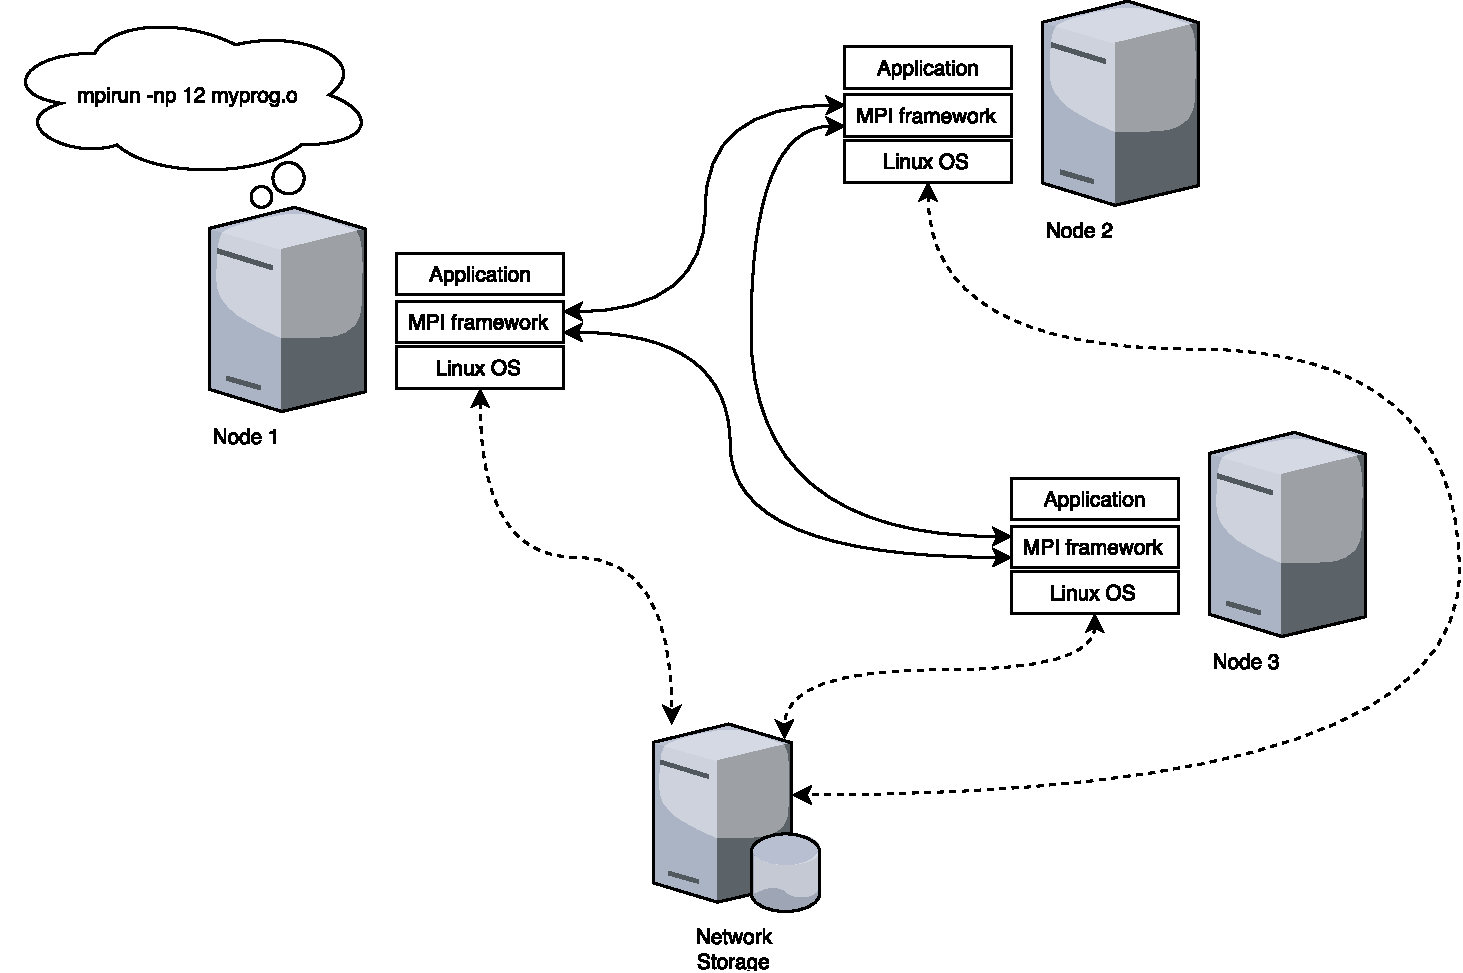
\includegraphics[scale=0.5]{img/cap1-mpiarchitecture.pdf}}
		\caption[MPI systems typical setup] {A typical configuration of MPI systems: the user launches the
		\texttt{mpirun} command on Node 1 that distributes the computation
		also over the Node 2 and Node 3. All nodes have access to a common 
		network storage to get the program and the data.}
		\label{fig:cap1-mpiarchitecture}
\end{figure}


\subsection{MPI Application Execution Flow}
A MPI typical MPI execution is presented in Figure 
\ref{fig:cap1-mpiarchitecture}. The user launches the job via the
\texttt{mpirun} command, then the MPI framework spawns the processes
in the other available machines (how this is performed is implementation
dependent).

The application must be linked with the static or dynamic library of MPI,
that provides \texttt{MPI\_*} function calls. Usually every program starts
with \texttt{MPI\_Init} and ends with \texttt{MPI\_Finalize}. Both functions
are implementation-dependent, but in general \emph{MPI\_Init} performs some
setup required before any other MPI routines and the
\texttt{MPI\_Finalize} coordinates the execution conclusion freeing the
allocated resources.

The communication between processes is divided in two categories:
\emph{point-to-point} (direct communication between two processes) and
\emph{collective}
(communication one-to-many or many-to-many). The latter is performed through
the coordination of the various MPI frameworks on all nodes. A typical example
of collective feature is the \emph{barrier}: every program should synchronize
at the same point before continuing.

Having a common set of functions allows to perform easily and equivalently
benchmarks of the same application on different MPI frameworks or to port
the program on another framework without refactoring the code.

\subsection{MPI implementations}

Today, several implementations of MPI are available, among which we cite
the two most commonly used: MPICH\cite{karonis2003mpich} and Open
MPI\cite{gabriel2004open}. They are both open source and have reached a good
level of stability even with a considerable number of features, thanks to the
very active communities and the large funding of big companies and
universities.

The history of MPICH can be split in two part: MPICH-1 and MPICH-2. The
development of the latter (at a later time called simply MPICH) starts in
2001 to add the feature of MPI version 2 and subsequently version 3 to MPICH-1.

Open MPI represents the union of three
previous implementations: LA-MPI, FT-MPI and LAM/MPI. The third 
was extensively used in research literature. All of which ceased their
development shortly after the begin of Open MPI project in 2003.

The two implementation mainly differs in the purpose of application: MPICH is
a very stable basis and standard reference for the development of special
purpose needs. Open MPI targets more general cases and it already offers
several pre-implemented features, e.g. different types of network
communication channels and topology.

Since our framework is supposed to be a general tool that tries to address
the issues of the most of HPC applications, we selected the Open MPI
implementation to develop the feature presented in next sections. Furthermore,
the extreme high modularity of Open MPI internal code was a big advantage in
the development of \texttt{mig} framework\footnote{Note that the keyword
`framework` may generate misunderstanding: as explained in Chapter
\ref{cap:design}, the \texttt{mig} framework is a module of Open MPI, not a new
MPI framework}.


\section{Migration of MPI processes}
This thesis presents a technique implemented in Open MPI able to allow the
migration of MPI processes among different nodes of the cluster. Moving a
process across different machines is not a straightforward task and
it constitutes a specific research topic. This work exploits existing
process migration tools applying them to Open MPI for HPC applications.

Migration of processes can be exploited to solve or mitigate some of the
previous presented issues. Obviously, the migration is not for free and
introduces an overhead that must
be taken in account, while being triggered by an appropriate software, for
instance by a fault detector or a resource manager.

Migration is particularly interesting for resource management: current runtime
resource managers in HPC are limited to assign resources during the application
startup, therefore they are not usually able to reschedule the application over
different nodes. Migration adds the capability of rescheduling to resource
managers, that they have to take in account the significant overhead of
moving processes between two nodes.

In large clusters the topology and consequently the location of the processes
of the same job significantly impacts on overall performance; even if
all nodes are in the same network, the distant of two machines noticeable
affects the network performance. If the topology of the cluster changes -
despite the application is not involved - a rescheduling may be convenient
to reach better performance. Since C/R is too expensive in terms of time and
required resources, this scenario can be an interesting exploitation of
migration techniques.

Regarding fault tolerance, the migration may in fact lead to a the reduction
of the number of C/R required:
an appropriate pre-fault detection system would trigger the migration if an
imminent fault is detected, avoiding the long restart required if the fault
happens.

Certainly, a sudden unexpected undetectable fault is not manageable with
a migration technique. This is why C/R mechanisms cannot be fully replaced.
Instead, the frequency of the checkpoints can be effectively reduced,
provided an appropriate fault probability analysis.

The software architecture considered for this work does not provide a fault
detector, but assume the presence of an external one that signals the resource
manager in case of imminent fault. Subsequently, the resource manager and the
MPI framework will trigger the migration. With this setup, the resource
manager is the only interlocutor with the MPI framework and it can allocate
and possibly reallocate resources over available nodes.

\section{Thesis structure and objectives}
The main topic of this thesis is a novel approach to process migration
implemented in Open MPI. This technique was also presented at the EuroMPI 2016
conference\cite{myEuroMPI}. In addition, the exploitation of this technique
with the \textbf{Barbeque Run-Time Resource Manager} (from now simply
\emph{BarbequeRTRM}) is presented in conjunction with a basic centralized
resource management policy for distributed systems.

In Chapter \ref{cap:state-of-the-art} the State of the art related to
migration and C/R techniques is discussed and the novelty of the
proposed method is highlighted. The Open MPI and CRIU frameworks are
described in Chapter \ref{cap:ompicriu}. Subsequently in Chapter
\ref{cap:design} and \ref{cap:integration} the design, the implementation and the integration with
\emph{BarbequeRTRM} are explained, detailing and arguing all design choices.
The testing results are discussed in Chapter \ref{cap:evaluation}, focusing on
the introduced overheads. Eventually, in Chapter \ref{cap:discussion} future
research directions and developments are proposed. It is also the thesis end containing the conclusions.   
 
\chapter{State of the Art}
\label{cap:state-of-the-art}

\section{Self-Adaptive Software Systems}
\label{sec:sas}
In modern-day applications, software complexity has extremely increased thanks to the spread of highly available and faster wireless connection such as in the Internet of Things (IoT) ambit. Since software is often deployed in dynamic contexts, where requirements, environment assumptions and usage profiles vary continuously, software complexity increased over time to the point where it is often composed by a number of sub-components and/or sub-services that work together in order to offer a service to the users. This is the case of service-oriented applications -- also called Service Based Systems (SBS) -- that are composed by multiple \emph{services} and \emph{components}. In these systems, services offered by third-party providers are dynamically composed into workflows to deliver complex functionalities, so SBSs rely on self adaptation to cope with the uncertainties associated with third-party services as the loose coupling of services makes a reconfiguration feasible. Without adaptation, the application is prone to degraded performance  because of faulty components, messages lost between services or delays due to an increasing number of users.

During the past decade a lot of research has been made in this scope but the engineering of adaptive systems remains an incredible challenge\cite{soft-eng-for-sas-2}. In order to solve the problem, \textbf{Self-Adapting Software Systems (SASS)} are born. These are flexible systems that can adapt themselves to their contextual needs and can do so with the highest performance and availability. General discussion concerning the issue and the state of the art in the design and implementation have been presented\cite{soft-eng-for-sas-2}\cite{survey-aut-comp}\cite{self-adap-soft}\cite{soft-eng-for-sas-1}\cite{soft-eng-for-sas-3}\cite{arch-based-appr-to-sas}\cite{sas-quant-ver}.

These kind of systems have some fundamental properties called auto-managing that are:
\begin{itemize}
	\item Auto-configuration
	\item Auto-recovery in case of failure
	\item Auto-optimization
	\item Auto-protection
\end{itemize}
All these properties can be grouped in two more abstract concepts which are self-awareness and context-awareness.

\textbf{Self-Awareness} is the ability of the system to be able to monitor itself in terms of available resources and behavior.

\textbf{Context-Awareness} is the ability of the system to understand the environment where it is working, using the information provided by its components, and adapt itself to all the changes that can occur during its normal operational status.
To better understand how a SASS works we need to answer some simple questions:
\begin{itemize}
	\item Who is adapting?
	\item What adaptation is required?
	\item When is it necessary to adapt?
	\item Where is it needed to change something?
	\item Why is it needed an adaptation?
	\item How do we achieve this goal?
\end{itemize}

During the past years have been developed some dimensions that help to answer all this simple questions: \emph{Time}, \emph{Reason}, \emph{Level}, \emph{Technique} and \emph{Adaptation Control} shown in Figure \ref{fig:dimensions}.
\begin{figure}[ht]
	\centerline
	{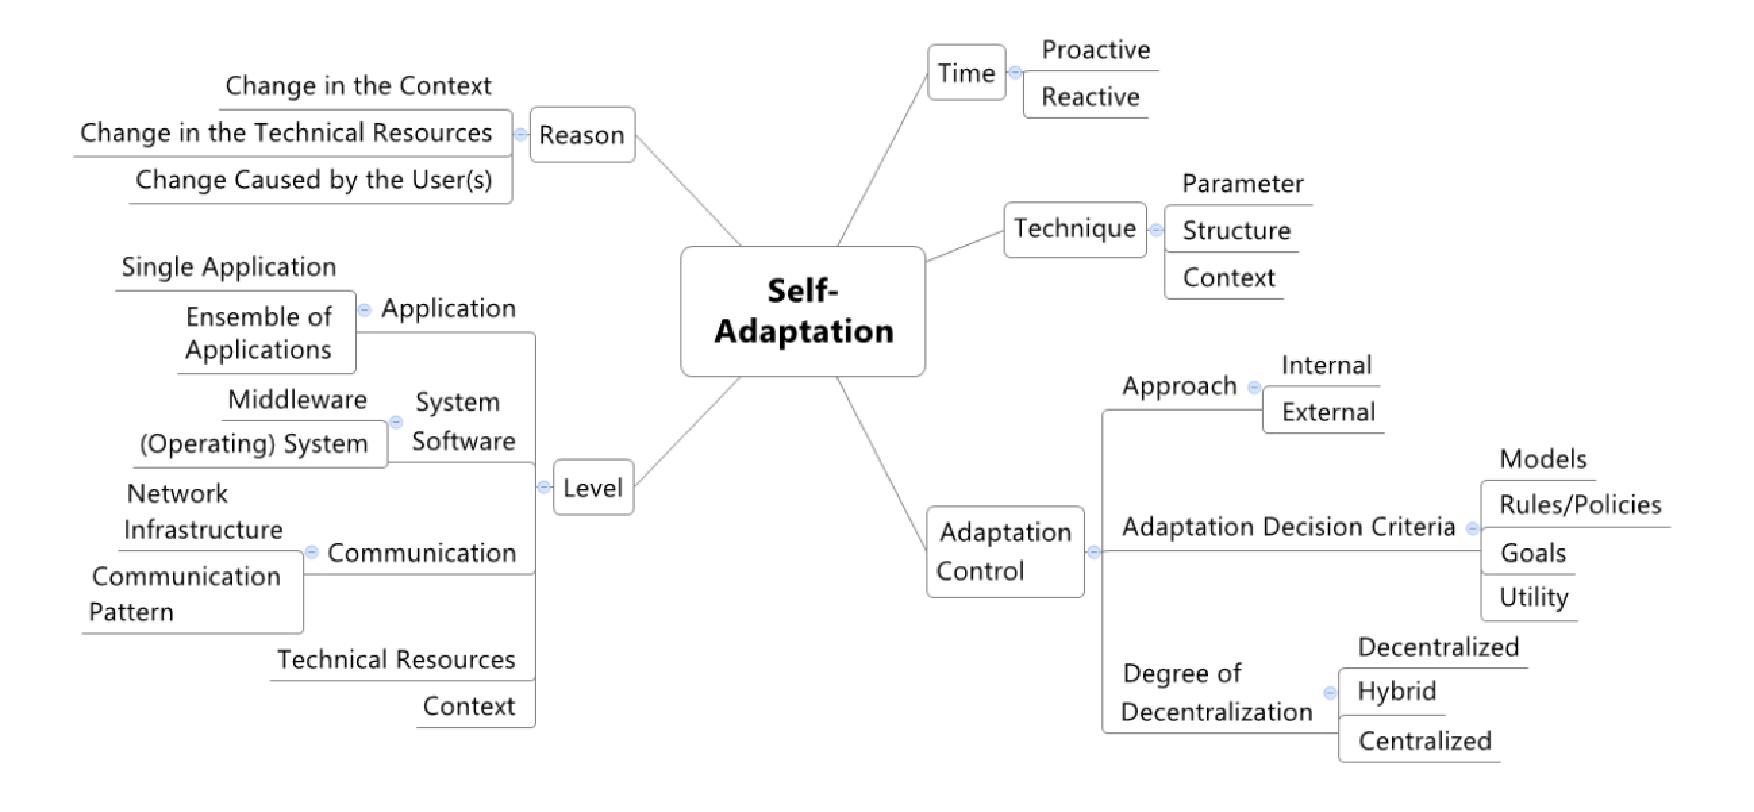
\includegraphics[scale=0.50]{img/dimensions.png}}
	\caption[The Dimensions]{The Dimensions to analyze adaptation.\cite{eng-appr-sas}}
	\label{fig:dimensions}
\end{figure}

\textbf{Who is adapting?} As the name suggests, it's the system itself that changes something in order to preserve some given constraint.

\textbf{What adaptation is required?} The \emph{Technique} dimension is the one that answers this question in fact the software engineer can change either the parameters or the system can be considered as a set of components. The former case allows to fine tuning the system at the expense of an higher complexity, the latter is called composite vision and permits the systems to cooperate exchanging algorithms and much more important, reusing components which improve performance because failed or defected components can be replaced.

\textbf{When it is necessary to adapt?} The \emph{Time} dimension is crucial in this situation. There are three typical approaches: the reactive one is the more traditional one which states that an adaptation is needed only after a causative event. The other two approaches are more interesting and they are predictive and proactive. The former studies the system before any event and calculate the need of an adaptation, the latter applies and adaptation despite an event and improves the performance. From the user perspective the proactive approach is the best because it doesn't interrupt the operation of the system in any load but it is the more complicated to implement. Monitoring continuously the system is a costly task to do, on the other side an adaptive monitoring is simple that analyze only specific aspect and/or resources and intervenes only if needed.

\textbf{Where it is needed to change something?} In general a SASS is composed by two main part: the the Adaptability Logic (AL) and the Managed Resource (MR). The former in general doesn't change, the latter is composed at the base of the hardware and of the software such as the operating system or, in case of distributed systems, the middleware that control the hardware; at a higher level of the application. These are the parts that require adaptation. To answer this question is needed to decide at which level the operation has to be applied without neglecting the relationship between the MR and the AL which is composed by the network that connects them and/or the view of the communication patterns. Thus \emph{Level} is the considered dimension.

\textbf{Why it is needed an adaptation?} In this case, \emph{Reason} is the right dimension. There can be one or more reason because a system needs adaptation such as a change in the available resources, a change in the environment or a change in the user base of the system.

\textbf{How do we achieve this goal?} The answer to this question is more complicated than the others because it needs a new topic called \emph{Adaptation Control}.

\subsection{Adaptation Control}
In the literature can be found 2 approaches: the \emph{internal approach} that intertwine the adaptation logic with the system resources, which has problems with the maintainability and scalability of the system, and the \emph{external approach} that splits the system into adaptation logic and managed resources, which increases maintainability and scalability through modularization.

The control unit needs a metric in order to decide how to adapt and in literature different metrics are present: models, rules and policies, goal or utility functions \cite{autonomic-computing}.

Another aspect of the adaptation logic is the degree of decentralization. If we have a system with limited resources then a centralized adaptation logic has to be preferred but with greater systems a decentralized AL can improve performance and  every sub-system can communicate with another with different patterns of communication. Of course hybrid technique can be made mixing the previous approaches.

\subsubsection{Adaptation Logic Issues}
As said before a SASS is composed of managed resources and the adaptation logic; it can be represented by the tuple \texttt{SASS = (AL, MR)}. \emph{AL = $a_1$, \dots, $a_n$}, with $a_i$ representing a logic element,  monitors the environment (M), analyzes the data for change (A), plans adaptation (P) and control the execution of the adaptation (E): these are known as \emph{MAPE cycle} or \emph{MAPE functionality}\cite{vision-aut-comp}. \emph{MR = $mr_1$, \dots, $mr_n$}, with $mr_i$ representing a resource, is the set of resources such as hardware with software, smart-phones, robotics or unmanned vehicles. Figure \ref{fig:sass} shows a SASS where the dashed line represent the system border.
\begin{figure}[ht]
	\centerline
	{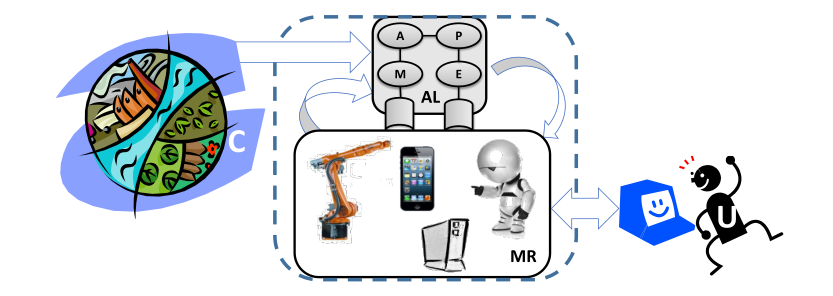
\includegraphics[scale=0.55]{img/managed-resources.png}}
	\caption[A SASS]{A SASS (AL = Adaptation Logic, MR = Managed Resources, U = User(s), C = Context, M,A,P,E = MAPE functionality).\cite{eng-appr-sas}}
	\label{fig:sass}
\end{figure}
The dimension can therefore be mapped to the MAPE functionalities as shown in table \ref{tab:mape}.
\begin{table}[ht!b]
	\centering
	\begin{tabular}{|l||p{2.4cm}|p{2.4cm}|p{2.4cm}|p{2.4cm}|}
		\hline 
		& \textbf{Time} & \textbf{Reason} & \textbf{Level} & \textbf{Technique} \\ 
		\hline 
		\textbf{Monitoring} & Continuos & What to monitor & Identification of the levels & --- \\ 
		\hline 
		\textbf{Analyzing} & Algorithms depend on reactive or proactive dimension & Where to analyze & --- & --- \\ 
		\hline 
		\textbf{Planning} & --- & What should be influenced by planning & Adaptation plans address these levels & Plans for performing the techniques \\ 
		\hline 
		\textbf{Executing} & --- & --- & Execution of the change on the levels & Execution of the change on the levels \\ 
		\hline 
	
	\end{tabular} 
\caption[MAPE and Dimensions]{Relation of the MAPE Activities and the Dimensions}
\label{tab:mape}
\end{table}

\section{The SOLAR Framework}
\label{sec:solar-framework}
Working on the adaptability of a system can impact other quality attributes such as performance, reliability or maintainability and in the worst case improving adaptability can decrease part, if not all, of these attributes as stated in \cite{bass2003software}: \emph{quality attributes can never be achieved in isolation, the achievement of any one will have an effect, sometimes positive and sometimes negative, on the achievement of others}.

Find a balance between these quality attributes is often a challenging task because sometimes they're conflicting each other, e.g. lower cost and higher availability, so find an adaptability value that can meet all the requisites is, as a consequence, a challenging task too.

The SOLAR (SOftware quaLities and Adaptability Relationships) framework \cite{solar} helps the software architect to select the best set of components in order to fulfill the requirements trying to achieve a minimum level for some quality attribute such as availability and/or cost. This tool helps the software architect to build a suitable architecture for his needs but is not a \emph{"solution for every situation"}.

\subsection{The SOLAR Metrics}
\label{subsec:solar-metrics}
All the metrics in SOLAR are greatly inspired by \cite{po-metrics} and are all defined at an architecture level and static perspective. 

To define them, the software architecture relies on a component-and-connector view (C\&C view). In this C\&C view \emph{components} are principal computational elements present at runtime. The representation used in Figure \ref{fig:comp-example} uses the UML diagram and shows some components and their respective connections.

\begin{figure}[ht]
	\centerline
	{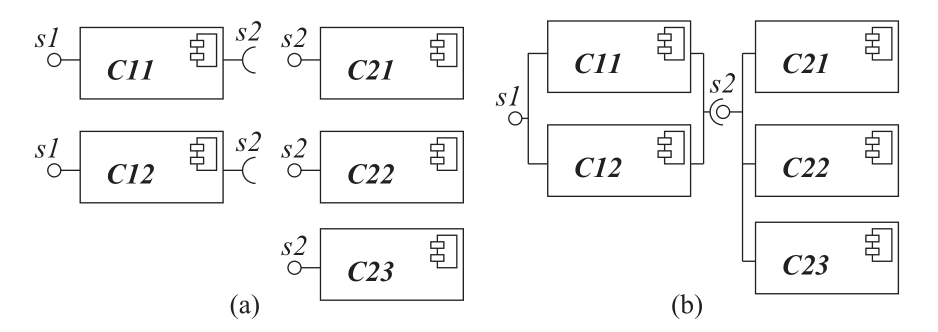
\includegraphics[scale=0.55]{img/solar-comp-example.png}}
	\caption[SOLAR Components example]{(a) A set of components and their interfaces and (b) the C\&C view of the components in (a)\cite{solar}.}
	\label{fig:comp-example}
\end{figure}

Components have interfaces attached to ports. \emph{Connectors} are pathways of interaction between components and also have interfaces or roles. In Figure \ref{fig:solar-arch-example} it is shown an example of an architecture, the used components are highlighted in gray; this example will be used to explain the metrics later in this chapter.

\begin{figure}[ht]
	\centerline
	{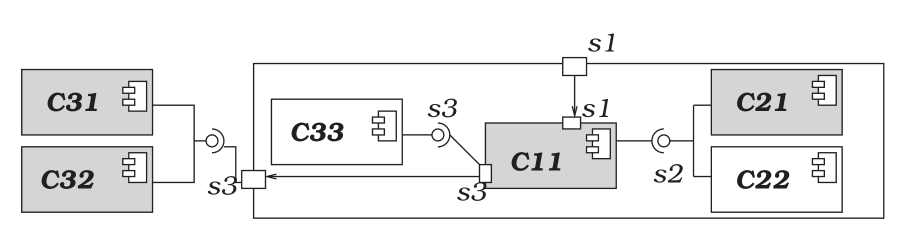
\includegraphics[scale=0.55]{img/solar-arch-example.png}}
	\caption[SOLAR example architecure]{C\&C view: discovered components and used components (in gray).\cite{solar}}
	\label{fig:solar-arch-example}
\end{figure}

In the architecture of Figure \ref{fig:solar-arch-example}:
\begin{itemize}
	\item the service S1 is provided by component C11 that is unique and must be in use. S1 is the provided service of this architecture.
	\item component C11 requires S2 and S3 services.
	\item service S2 is provided by C21 and C22 where only C21 is in use.
	\item service S3 is provided by C31, C32 and C33 but only C31 and C32 are in use.
\end{itemize}

\subsubsection{Absolute adaptability of a service (AAS)}
This metric measures the number of used components for providing a given service.
\[ AAS \in \mathbb{N}^n |AAS_i = |UC_i|\]
Quantifies how much adaptable a service is by counting the different alternatives to execute the service (1 no adaptable, $>$1 adaptable), where the service adaptability grows according to the number of components able to provide it. 

\noindent Referring to the example in Figure \ref{fig:solar-arch-example}, we observe that $AAS = [1, 1, 2]$.

\subsubsection{Relative adaptability of a service (RAS)}
This metric measures the number of used components that provide a given service with respect to the number of components actually offering such service.
\[ RAS \in \mathbb{Q}^n | RAS_i = \frac{|UC_i|}{|C_i|} \]
It describes how each service stresses its adaptability choices and it informs how much more adaptable the service could be. RAS vector values near to one mean that the service is using almost all the adaptability potentially reachable. 

\noindent Referring to the example in Figure \ref{fig:solar-arch-example}, we observe that $RAS = [1, 0.5, 0.6]$.

\subsubsection{Mean of absolute adaptability of services (MAAS)}
This metric measures the mean number of used components per service.
\[ MAAS \in \mathbb{Q} | MAAS = \frac{\sum_{i=1}^{n} AAS_i}{n}  \]
It offers insights into the mean size and effort needed to manage each service.

\noindent Referring to the example in Figure \ref{fig:solar-arch-example}, $MAAS = 4/3 = 1.3$. 

Architectures with more adaptable services have higher values of MAAS. Besides, a $MAAS > 1$ means that the architecture includes adaptable services (at least one of the components $AAS_i > 1$). For $MAAS \le 1$, there may be adaptable services or not (AAS should be checked in this case).

\subsubsection{Mean of relative adaptability of services (MRAS)}
This metric represents the mean of RAS.
\[ MRAS \in \mathbb{Q} | MRAS = \frac{\sum_{i=1}^{n}RAS_i}{n}\]
It informs about the mean utilization of the potential components for each service. Values of this metric range between zero and one.

\noindent Referring to the example, $MRAS = (1 + 0.5 + 0.6)/3 = 0.72$.

The higher the MRAS of an architecture, the more adaptable its services are, on average. The maximum value of this metric is obtained when $RAS_i = 1 \;\;\forall i \in [1, \dots, n]$, which is in turn obtained when all services are as much adaptable as possible because they use all the available components. Therefore, a value close to one for MRAS means that, on average, services are as much adaptable as possible. A value close to zero means that: 
\begin{enumerate}
	\item[\textbf{a)}] services can be much more adaptable (adding components not yet used)
	\item[\textbf{b)}] different architecture alternatives with the same quantity of adaptability can be created
\end{enumerate}

\subsubsection{Level of system adaptability (LSA)}
This metric measures the number of components used to make up the system with respect to the number of components that the most adaptable architecture would use.
\[ LSA \in \mathbb{Q}{0..1} | LSA = \frac{\sum_{i=1}^{n}AAS_i}{\sum_{i=1}^{n}|C_i|} \]
The value of this metric ranges between zero and one. For LSA, a value of one means that the system is using all existing components for each service, i.e., $AAS_i = |C_i | \forall i \in {1,\dots, n}$, and then its adaptability is already to the maximum. A value close to one means that the market offers few choices to increase the system architectural adaptability. When a new component is bounded to the architecture, LSA increases in a constant value ($1/\sum{{i=1}^{n}|C_i}$) irrespective of the number of components already considered for the same service.

\noindent Referring to the example in Figure \ref{fig:solar-arch-example}, $LSA = 4/(1 + 2 + 3) = 0.6$.

Table \ref{tab:solar-metrics-summary} summarizes the five metrics and their values for the example in Figure \ref{fig:solar-arch-example}.

\begin{table}[ht!b]
	\centering
	\begin{tabular}{|l|l|l|l|}
		\hline 
		Name & Range & Value & Example in Fig. \ref{fig:solar-arch-example} \\ 
		\hline 
		AAS & $\mathbb{N}^n$ & ${|UC_i|}$ & $[1,1,2]$ \\

		RAS & $\mathbb{Q}^n \in {0,\dots,1}$ & ${\frac{|UC_i|}{|C_i|}}$ & $[1,0.5,0.6]$ \\ 

		MAAS & $\mathbb{Q}_+$ & $\frac{\sum_{i=1}^{n}AAS_i}{n}$ & $1.3$ \\ 

		MRAS & $\mathbb{Q}^n \in {0,\dots,1}$ & $\frac{\sum_{i=1}^{n}RAS_i}{n}$ & $0.72$ \\ 
		
		LSA & $\mathbb{Q}^n \in {0,\dots,1}$ & $\frac{\sum_{i=1}^{n}AAS_i}{\sum_{i=1}^{n}|C_i|}$ & $0.6$ \\
		\hline 
		
	\end{tabular} 
	\caption[SOLAR Metrics]{Summary of the metrics.\cite{solar}}
	\label{tab:solar-metrics-summary}
\end{table}

\subsection{Relating adaptability to a system quality attribute}
The analysis of the relation between system adaptability and quality attributes can give three different results as shown in Table \ref{tab:adapt-qual}.  In the rows we read that, when the adaptability increases then some quality attributes:
\begin{itemize}
	\item tend to increase their measured values
	\item tend to decrease their measured values
	\item are not affected. We are not interested in this group since we are focussed on the influence of adaptability on the requirement.
\end{itemize}

\noindent The columns in the table consider how the quality requirement is formulated:
\begin{itemize}
	\item as higher than, e.g., "system availability shall be higher than\dots"
	\item as lower than, e.g., "system mean response time shall be lower than\dots"
\end{itemize}

Each region of interest in Table \ref{tab:adapt-qual} has been labeled as Helps or Hurts to indicate the effect of the adaptability upon the quality requirement. 

\noindent The best cases are when the quality attribute completely depends on the adaptability such as:
\begin{enumerate}
	\item The higher the adaptability, the higher the quality attribute
	\item The lower the adaptability, the lower the quality attribute
\end{enumerate}

In Figure \ref{fig:solar-inter-cases} are shown all the intermediate cases that can result mixing the two extreme cases above. The \emph{X} axis represents the adaptability value, The \emph{Y} axis represent the quality attribute. For each value of adaptability there are two extreme values:
\begin{itemize}
	\item $Q_{A_iU}$ is the maximum value of the quality attribute with respect to $A_i$
	\item $Q_{A_iL}$ is the minimum value of the quality attribute with respect to $A_i$
\end{itemize} 
Between these extreme values there are all the architecture that have the same adaptability and intermediate quality attribute value. Among all the $Q_{A_iU}$ and $Q_{A_iL}$ in the graph, two of them have a particular meaning: $Adapt^+$ and $Adapt^-$.

To describe the meaning of $Adapt^-$ and $Adapt^+$ we focus on parts (a) and (d) in Figure \ref{fig:solar-inter-cases}. $Adapt^-$ is the lowest $A_i$ for which we can find an architecture satisfying the requirement. $Adapt^+$ is the lowest $A_i$ whose bounds, $Q_{A_iU}$ and $Q_{A_iL}$, satisfy the requirement. These values indicate that to fulfill the requirement, the architecture must have at least adaptability $Adapt^-$, and, any architecture with at least $Adapt^+$ will also satisfy it. For adaptabilities between them, there will be architectures satisfying the requirement (those highlighted in the figure) and others that will not. 

In parts (b) and (c) in Figure \ref{fig:solar-inter-cases} (regions where the adaptability Hurts), $Adapt^-$ is the threshold adaptability value for which any architecture with adaptability $A_i \le Adapt^-$ fulfills the requirement; and $Adapt^+$ is the maximum $A_i$ for which we know that exists some architecture that satisfies the requirement.

\begin{table}[ht!b]
	\centering
	\begin{tabular}{lx{3cm}x{3cm}}
		\firsthline
		\multirow{2}{*}{When adaptability increases} & \multicolumn{2}{c}{Requirement formulated as} \\
		\cline{2-3}
		& \emph{Higher than} & \emph{Lower than} \\
		\hline
		The quality attribute value increases & Helps & Hurts \\
		The	quality attribute value decreases & Hurts & Helps \\
		The	quality attribute is not affected & \multicolumn{2}{c}{No effect}\\
		\hline
	\end{tabular}
	\caption[Adaptability w.r.t. quality requirements]{Effect of adaptability on a measured quality requirement.\cite{solar}}
	\label{tab:adapt-qual}
\end{table}
\begin{figure}[ht]
	\centerline
	{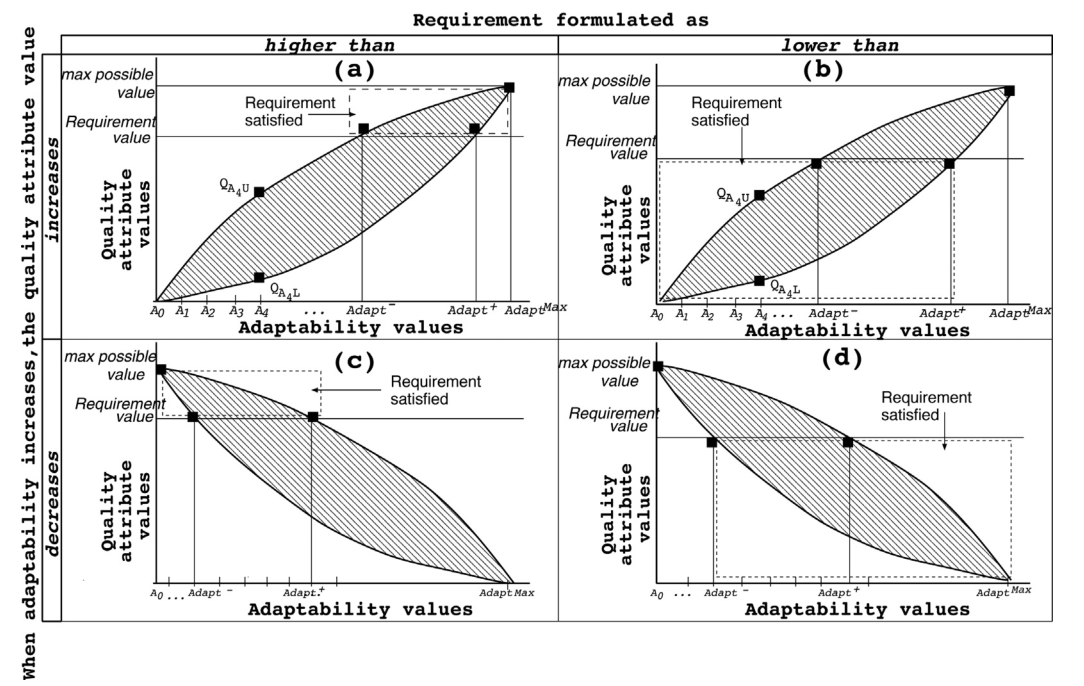
\includegraphics[scale=0.55]{img/solar-inter-cases.png}}
	\caption[Relations among adaptability and other quality attributes.]{Relations among adaptability and other quality attributes.\cite{solar}}
	\label{fig:solar-inter-cases}
\end{figure} 
\subsection{Analysis of the approach and its limits}
Both of these tools want to help the software architect in choosing the right set of components in order to satisfy the adaptability requirements and if possible other quality attributes. With the SOLAR framework all the possible architectures that satisfy the requisites are generated and the choice is left to the architect. This approach is for sure slower but is a valid tool to have an idea of the possible outcome and build an architecture from scratch. On the other side it presents some limitations presented in no particular order:
\begin{itemize}
	\item It analyzes all the architecture only with a static analysis using the component diagram.
	\item All components are given equal importance thus the time a component is used and the number of usages per call is completely ignored.
	\item It does not considers the probability of failure of a component at runtime.
	\item Requires a lot of time to produce complete results.
\end{itemize}
In the next chapter it is shown how to analyze the quality of a software and in particular how to evaluate the adaptability of a software with respect to some attributes such as cost and availability.


\begin{appendices}

\end{appendices}


\cleardoublepage
\phantomsection
\addcontentsline{toc}{chapter}{\bibname}
\small
\bibliographystyle{unsrt}
\bibliography{thesis}



\end{document}
